%%%%%%%%%%%%%%%%%%%%%%%%%%%%%%%%%%%%%%%%%%%%%%%%%%%%%%%%%%%%%%%%%%%%%%%%%%%%%%%%%%%%%%%%%%%%%%%%
%
% CS484 Written Question Template
%
% Acknowledgements:
% The original code is written by Prof. James Tompkin (james_tompkin@brown.edu).
% The second version is revised by Prof. Min H. Kim (minhkim@kaist.ac.kr).
%
% This is a LaTeX document. LaTeX is a markup language for producing 
% documents. Your task is to fill out this document, then to compile 
% it into a PDF document. 
%
% 
% TO COMPILE:
% > pdflatex thisfile.tex
%
% If you do not have LaTeX and need a LaTeX distribution:
% - Personal laptops (all common OS): www.latex-project.org/get/
% - We recommend latex compiler miktex (https://miktex.org/) for windows,
%   macTex (http://www.tug.org/mactex/) for macOS users.
%   And TeXstudio(http://www.texstudio.org/) for latex editor.
%   You should install both compiler and editor for editing latex.
%   The another option is Overleaf (https://www.overleaf.com/) which is 
%   an online latex editor.
%
% If you need help with LaTeX, please come to office hours. 
% Or, there is plenty of help online:
% https://en.wikibooks.org/wiki/LaTeX
%
% Good luck!
% Min and the CS484 staff
%
%%%%%%%%%%%%%%%%%%%%%%%%%%%%%%%%%%%%%%%%%%%%%%%%%%%%%%%%%%%%%%%%%%%%%%%%%%%%%%%%%%%%%%%%%%%%%%%%
%
% How to include two graphics on the same line:
% 
% \includegraphics[width=0.49\linewidth]{yourgraphic1.png}
% \includegraphics[width=0.49\linewidth]{yourgraphic2.png}
%
% How to include equations:
%
% \begin{equation}
% y = mx+c
% \end{equation}
% 
%%%%%%%%%%%%%%%%%%%%%%%%%%%%%%%%%%%%%%%%%%%%%%%%%%%%%%%%%%%%%%%%%%%%%%%%%%%%%%%%%%%%%%%%%%%%%%%%

\documentclass[11pt]{article}

\usepackage[english]{babel}
\usepackage[utf8]{inputenc}
\usepackage[colorlinks = true,
linkcolor = blue,
urlcolor  = blue]{hyperref}
\usepackage[a4paper,margin=1.5in]{geometry}
\usepackage{stackengine,graphicx}
\usepackage{fancyhdr}
\setlength{\headheight}{15pt}
\usepackage{microtype}
\usepackage{times}

% From https://ctan.org/pkg/matlab-prettifier
\usepackage[numbered,framed]{matlab-prettifier}

\frenchspacing
\setlength{\parindent}{0cm} % Default is 15pt.
\setlength{\parskip}{0.3cm plus1mm minus1mm}

\pagestyle{fancy}
\fancyhf{}
\lhead{Homework 2 Questions}
\rhead{CS484}
\rfoot{\thepage}

\date{}

\title{\vspace{-1cm}Homework 2 Questions}


\begin{document}
	\maketitle
	\vspace{-3cm}
	\thispagestyle{fancy}
	
	\section*{Instructions}
	\begin{itemize}
		\item 4 questions.
		\item Write code where appropriate.
		\item Feel free to include images or equations.
		\item \textbf{Please use only the space provided and keep the page breaks.} Please do not make new pages, nor remove pages. The document is a template to help grading.
		\item If you really need extra space, please use new pages at the end of the document and refer us to it in your answers.
	\end{itemize}

	\section*{Questions}
	
	\paragraph{Q1:} Explicitly describe image convolution: the input, the transformation, and the output. Why is it useful for computer vision?
	
	%%%%%%%%%%%%%%%%%%%%%%%%%%%%%%%%%%%
	\paragraph{A1:} Your answer here.
	
	In image processing, convolution is the process of transforming an image by applying a kernel (input 1) over each pixel and its local neighbors across the entire image (input 2). Ensuring the kernel is in within the image, Convolution Process places the kernel over each pixel of the image and multiplies each value of the kernel with the corresponding pixel it is over and sums the resulting multiplied values and return the resulting value as the new value of the center pixel. We repeat this process across the entire image. The output of the process changes as we change the input kernel. Convolution is indeed very useful since we can extract certain desired features from the image by choosing an appropriate kernel. It is a key concept in CNNs. In its convolution level, CNN applies convolution on its inputs using a Kernel Matrix that it calibrates through training. For this reason, CNNs are very good at feature matching in images and object classification.
	
	
	%%%%%%%%%%%%%%%%%%%%%%%%%%%%%%%%%%%
	
	% Please leave the pagebreak
	\pagebreak
	\paragraph{Q2:} What is the difference between convolution and correlation? Construct a scenario which produces a different output between both operations.
	
	\emph{Please use \href{https://www.mathworks.com/help/images/ref/imfilter.html}{$imfilter$} to experiment! Look at the `options' parameter in MATLAB Help to learn how to switch the underlying operation from correlation to convolution.}
	
	%%%%%%%%%%%%%%%%%%%%%%%%%%%%%%%%%%%
	\paragraph{A2:} Your answer here.
	
	Both, convolution and correlation filtering, are linear filtering. However, there is a small difference between them. We use the filter without making any further changes on it in correlation filtering. On the other hand, for the convolution filtering, we have to flip the filter bottom to top and right  to left (180 degree). To have a scenario where these 2 different methods produce different outputs, we have to make sure that our filter is not symmetric, otherwise rotation would not affect it. As an example, we run the following Matlab code where we apply the "Sobel" filter to see the difference.
	
	\begin{lstlisting}[style=Matlab-editor]
    genius=imread('../data/einstein.bmp');
    sobel=[1,2,1;0,0,0;-1,-2,-1];
    correlation = imfilter(genius,sobel);
    convolution = imfilter(genius,sobel,'conv');
    figure(1);
    imshow(correlation);
    figure(2);
    imshow(convolution);
    \end{lstlisting}
	
	We get the following ouputs:
	
	\begin{figure}[htp]
    \centering
    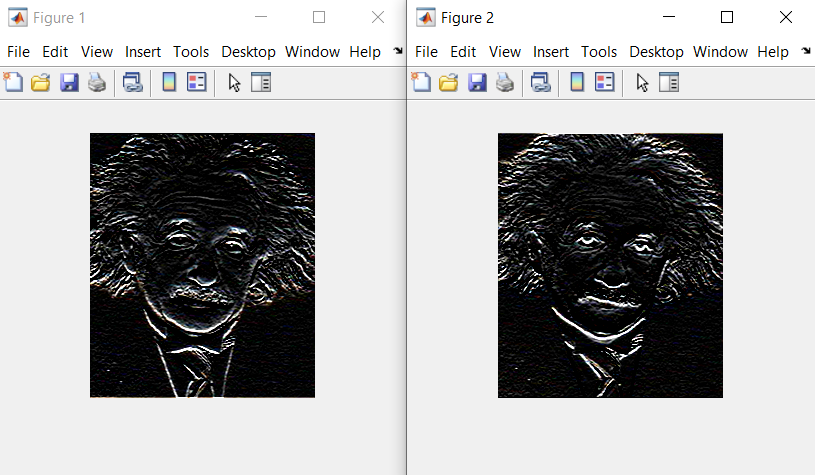
\includegraphics[width=10cm]{questions/EinsteinResult.PNG}
    \caption{Results of Correlation and Convolution filters, respectively.}
    \label{fig:einstein}
    \end{figure}
	
	
	
	%%%%%%%%%%%%%%%%%%%%%%%%%%%%%%%%%%%
	
	% Please leave the pagebreak
	\pagebreak
	\paragraph{Q3:} What is the difference between a high pass filter and a low pass filter in how they are constructed, and what they do to the image? Please provide example kernels and output images.
	
	%%%%%%%%%%%%%%%%%%%%%%%%%%%%%%%%%%%
	\paragraph{A3:} Your answer here.
	
	The high pass frequency components denotes edges whereas the low pass frequency components denotes smooth regions.
	
	Common example of low pass filter: When one is placed inside and the zero is placed outside , we got a blurred image. Now as we increase the size of 1, blurring would be increased and the edge content would be reduced.It is used for smoothing the image. It attenuates the high frequency.
	
	Common example of high pass filter: When 0 is placed inside, we get edges, which gives us a sketched image. An ideal low pass filter in frequency domain is given below.It is used for sharpening the image. It attenuates the low frequency 
	
	We use the following low pass filter to smooth the image. And we substract this image from the original one to get the high frequencies.
	
	\begin{lstlisting}[style=Matlab-editor]
    filter = fspecial('Gaussian', 29, 7);
    \end{lstlisting}
    
    Result: 
    
    \begin{figure}[htp]
    \centering
    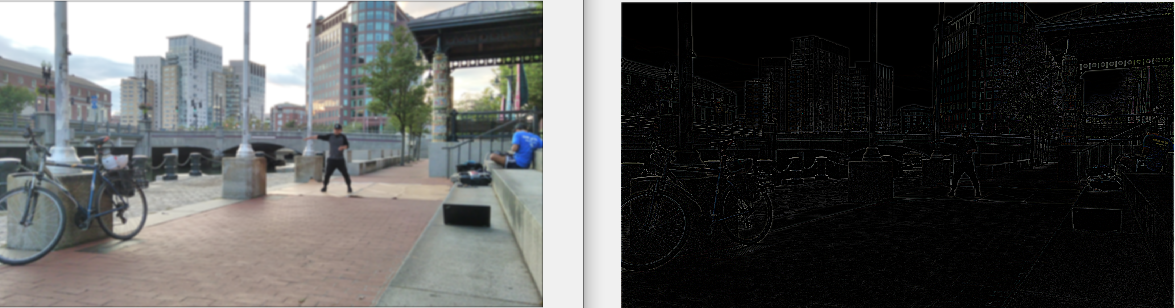
\includegraphics[width=15cm]{questions/nenene.PNG}
    \caption{Result of low-pass and high-pass filtering, respectively}
    \label{fig:einstein}
    \end{figure}
	
	
	%%%%%%%%%%%%%%%%%%%%%%%%%%%%%%%%%%%
	
	% Please leave the pagebreak
	\pagebreak
	\paragraph{Q4:} How does computation time vary with filter sizes from $3\times3$ to $15\times15$ (for all odd and square sizes), and with image sizes from 0.25~MPix to 8~MPix (choose your own intervals)? Measure both using \href{https://www.mathworks.com/help/images/ref/imfilter.html}{$imfilter$} to produce a matrix of values. Use the \href{https://www.mathworks.com/help/images/ref/imresize.html}{$imresize$} function to vary the size of an image. Use an appropriate charting function to plot your matrix of results, such as \href{https://www.mathworks.com/help/matlab/ref/scatter3.html}{$scatter3$} or \href{https://www.mathworks.com/help/matlab/ref/surf.html}{$surf$}.
	
	Do the results match your expectation given the number of multiply and add operations in convolution?
	
	See RISDance.jpg in the attached file.
	
	%%%%%%%%%%%%%%%%%%%%%%%%%%%%%%%%%%%
	\paragraph{A4:} Your answer here.
	 We run the code in scatter.m file in 'code' file, to get the following plot.
	 \begin{figure}[htp]
    \centering
    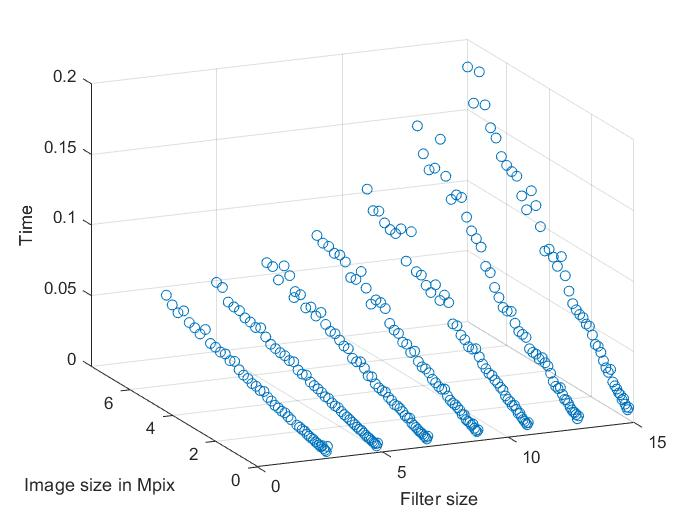
\includegraphics[width=10cm]{questions/scatter.jpg}
    \caption{Computation variation plot}
    \label{fig:einstein}
    \end{figure}
	
	We see that both filter size and image size affect the running time of our code. Running time increases as we increase filter and images sizes. The bigger the filter size, longer it takes. The bigger the image size, the longer it  takes. 
	
	%%%%%%%%%%%%%%%%%%%%%%%%%%%%%%%%%%%
	
	
	% If you really need extra space, uncomment here and use extra pages after the last question.
	% Please refer here in your original answer. Thanks!
	%\pagebreak
	%\paragraph{AX.X Continued:} Your answer continued here.
	
	
	
\end{document}